\problemname{Grid Delivery}

Your friend Ellie owns a local parcel delivery business called Grid City 
Parcel Courier (GCPC) which operates in Grid City, a town where all houses are
aligned on a rectangular grid of streets. Each house is placed at the intersection
of two streets, one running in north-south direction (vertically) and one
running in east-west direction (horizontally). There are $w$ vertical streets and
$h$ horizontal streets, resulting in a $h\times w$ grid of houses.

To grow her business, Ellie wants to start offering parcel pickup too.
However, the mayor of Grid City recently decided that all streets will 
be one-way streets during the day to combat traffic jams. During this time,
the streets of Grid City can only be passed from north to south or west to
east, respectively.

\begin{figure}[!h]
  \centering
	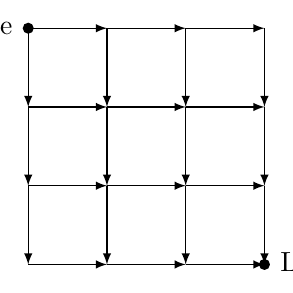
\begin{tikzpicture}
		\draw[-latex] (0,3) -- (1,3);
		\draw[-latex] (1,3) -- (2,3);
		\draw[-latex] (2,3) -- (3,3);
		\draw[-latex] (0,2) -- (1,2);
		\draw[-latex] (1,2) -- (2,2);
		\draw[-latex] (2,2) -- (3,2);
		\draw[-latex] (0,1) -- (1,1);
		\draw[-latex] (1,1) -- (2,1);
		\draw[-latex] (2,1) -- (3,1);
		\draw[-latex] (0,0) -- (1,0);
		\draw[-latex] (1,0) -- (2,0);
		\draw[-latex] (2,0) -- (3,0);
		\draw[-latex] (0,3) -- (0,2);
		\draw[-latex] (0,2) -- (0,1);
		\draw[-latex] (0,1) -- (0,0);
		\draw[-latex] (1,3) -- (1,2);
		\draw[-latex] (1,2) -- (1,1);
		\draw[-latex] (1,1) -- (1,0);
		\draw[-latex] (2,3) -- (2,2);
		\draw[-latex] (2,2) -- (2,1);
		\draw[-latex] (2,1) -- (2,0);
		\draw[-latex] (3,3) -- (3,2);
		\draw[-latex] (3,2) -- (3,1);
		\draw[-latex] (3,1) -- (3,0);

		\useasboundingbox (current bounding box);

		\node[circle,fill=black,inner sep=0pt,minimum size=4pt,label=left:{Garage}] at (0,3) {};
		\node[circle,fill=black,inner sep=0pt,minimum size=4pt,label=right:{Logistics Center}] at (3,0) {};
	\end{tikzpicture}
	\caption{Visualization of the grid of one-way streets given in the first sample input.}
\end{figure}

Ellie already rented a large garage located at the city's northwesternmost
intersection, from which her drivers will start their journeys to collect
parcels. She asked you to help her figure out how many drivers she needs to
hire to collect all parcels during the day and bring them to her logistics
center located at the city's southeasternmost intersection.

\section*{Input}
The input consists of:
\begin{itemize}
	\item One line with two integers $h$ and $w$ ($1 \le h,w \le 2\,000$),
		the height and width of the grid.
	\item $h$ lines, each with $w$ characters which are either
		\texttt{C}, indicating the house of a customer where a parcel has to 
		be collected, or \texttt{\_}, indicating a house where nothing has 
		to be collected.
\end{itemize}

\section*{Output}
Output the minimal number of drivers required to collect all parcels 
while all streets are one-way streets.
